\section{Change of object's location over time}
\label{sec-change-location}

\textbf{Created by:} Arkopaul Sarkar \\
\textbf{Modified by:} Arkopaul Sarkar \\

\subsection*{Scenario Objective}

This scenario illustrates how to represent the change in an object's physical location over time using the IOF/BFO ontology framework. It focuses on:
\begin{itemize}
    \item Emphasizing physical locations as sites and their association with spatial regions.
    \item Capturing actual movements of objects between existing locations (does not express any future plan or schedule of movement).
    \item \textbf{Temporal focus:} Associating specific temporal instants with the object's presence at particular locations.
\end{itemize}

\subsection*{General Pattern Description}
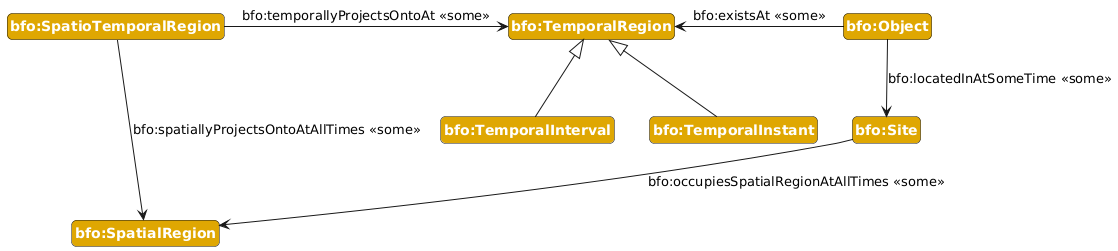
\includegraphics[scale=0.38]{scenarios/location-change/images/change-of-location-general.png}

An object may be located in different places at different times. In this scenario, the object can be related to multiple locations as \texttt{bfo:Site} by \texttt{bfo:locatedInAtSomeTime} property. Similarly, the object can be related to multiple \texttt{bfo:TemporalRegion}, each being either \texttt{bfo:TemporalInterval} or \texttt{bfo:TemporalInstant} by \texttt{bfo:existsAt}. As the object cannot be at two different locations at the same time, the times and the locations need to be paired up to denote at which location the object was at what time. This pairing can be done by different \texttt{bfo:SpationTemporalRegion}. Following the 4D ontology of BFO, the object's spatial and temporal co-occupation can be represented by a \texttt{bfo:SpationTemporalRegion}, which \texttt{bfo:temporallyProjectsOnto} the temporal region the object exists at and \texttt{bfo:spatiallyProjectsOntoAtAllTimes} the \texttt{bfo:SpatialRegion} the object occupies (\texttt{occupiesSpatialRegionAtAllTimes}). 

Note that the pattern shows that it is the object's location (a \texttt{bfo:Site}) that \texttt{occupiesSpatialRegion\\AtAllTimes}. However, an object also occupies the same spatial region that its location occupies. Therefore, this pattern can also be used by directly relating the object to a spatial region by \texttt{occupiesSpa\\tialRegionAtAllTimes}. The choice depends on the kind of location, which is detailed in \cref{?chapter-space-location}.   

Note further that a \texttt{SpatioTemporalRegion} cannot project onto two or more different \texttt{bfo:SpatialRegio\\n}s while projecting on a single \texttt{bfo:TemporalRegion}, as an object cannot be at two different locations at the same time. But it can be in the same location at different times. Therefore, a \texttt{SpatioTemporalRegion} can project onto two or more different \texttt{bfo:TemporalRegion} while projecting on a single \texttt{bfo:SpatialReg\\ion}. However, the data mapping becomes easier if one pair of temporal and spatial regions is related to each spatio-temporal region. If the object is in the same location at different times, two spatio-temporal regions can relate each temporal region to the same spatial region. Observe that these two spatio-temporal regions are simply parts of the spatio-temporal region that projects onto two temporal regions. Therefore, they capture the same semantics while making data mapping easier.     

\subsubsection*{Use Case: Freight Train Location Change} 
A freight train operated by BNSF Railway hauls coal from Powder River Basin, Wyoming, to the Port of Long Beach in California. It was located at Powder River Basin station at 11:00 AM on Wednesday and then at Long Beach station at midnight on Thursday.

\subsubsection*{Use-Case Pattern Description}
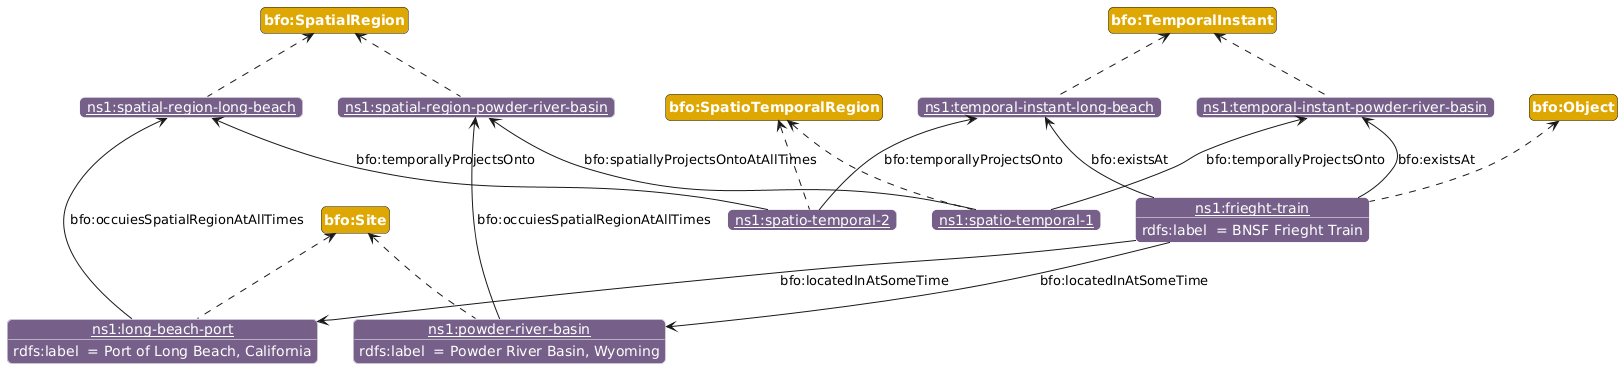
\includegraphics[scale=0.27]{scenarios/location-change/images/change-of-location-usecase1.png}
\begin{itemize}
    \item The train \texttt{ns1:freight-train} is located at (\texttt{bfo:locatedInAtSomeTime}) two different locations: \texttt{ns1:powder-river-basin} and \texttt{ns1:long-beach-port}, both of which are instances of \texttt{bfo:site}.
    \item Two separate instances of \texttt{bfo:SpatialRegion}: \texttt{ns1:spatial-region-powder-river-basin} and \texttt{ns1:spatial-region-long-beach}.
    \item The sites are linked to the spatial regions by \texttt{occupiesSpatialRegionAtAllTimes}.
    \item Temporal instants are linked to the sites, but the actual clock times are omitted for brevity.
\end{itemize}

\subsubsection*{Use-Case Example Data}

\begin{tabularx}{\textwidth}{|X|l|X|X|X|}
\hline
Train Number & Source & Destination & Departure Time & Arrival Time \\
\hline
1            & Powder River Basin & Long Beach      & 11:00 AM      & Midnight       \\
2            & Example Source     & Example Dest    & 10:00 AM      & 2:00 PM        \\
3            & Example Source 2   & Example Dest 2  & 8:00 AM       & 4:00 PM        \\
\hline
\end{tabularx}

\subsubsection*{Data Mapping Description}

\begin{verbatim}
INSERT DATA {
    <http://example.org/ns1:freight-train> a <http://example.org/bfo:Entity>;
    <http://example.org/ns1:freight-train> <http://example.org/bfo:locatedInAtSomeTime> 
        <http://example.org/ns1:powder-river-basin>.
}
\end{verbatim}

\subsubsection*{Data Validation}